% !TEX TS-program = pdflatex
% !TEX encoding = UTF-8 Unicode
\documentclass[a4paper]{article}
\usepackage[english]{babel}
\usepackage[T1]{fontenc}
\usepackage[utf8]{inputenc}
\usepackage{mathtools}
\usepackage[pdftex]{graphicx}
\usepackage{float}
\usepackage{fancyhdr}
\usepackage{geometry}
\usepackage{booktabs} % for much better looking tables
\usepackage{array} % for better arrays (eg matrices) in maths
\usepackage{paralist} % very flexible & customisable lists (eg. enumerate/itemize, etc.)
\usepackage{verbatim} % adds environment for commenting out blocks of text & for better verbatim
\usepackage{subfig} % make it possible to include more than one captioned figure/table in a single float

%%% HEADERS & FOOTERS

\author{Jonathan Karlsson - jonka293 - 890201-1991 \and Niclas Olofsson - nicol271 - 900904-5338}
\pagestyle{fancy} % options: empty , plain , fancy
\renewcommand{\headrulewidth}{1pt} % customise the layout...
\fancyhead[LO,LE]{Laboration 4 - TDDC78}
\lfoot{}\cfoot{\thepage}\rfoot{}
\setlength{\parindent}{0pt}

%%%% SECTION TITLE APPEARANCE

%\usepackage{sectsty}
%\allsectionsfont{\sffamily\mdseries\upshape} % (See the fntguide.pdf for font help)
%% (This matches ConTeXt defaults)
%
%%%% ToC (table of contents) APPEARANCE
%\usepackage[nottoc,notlof,notlot]{tocbibind} % Put the bibliography in the ToC
%\usepackage[titles,subfigure]{tocloft} % Alter the style of the Table of Contents
%\renewcommand{\cftsecfont}{\rmfamily\mdseries\upshape}
%\renewcommand{\cftsecpagefont}{\rmfamily\mdseries\upshape} % No bold!

%%% END Article customizations

%%% The "real" document content comes below...

\title{Laboration 4 - TDDC78}

%\date{} % Activate to display a given date or no date (if empty),
% otherwise the current date is printed

\begin{document}

\maketitle

\section{Program description}
This program simulates a number of particles with a certain initial
speed and position, moving inside a box. Particles can collide with each
other, and with the walls of the box. Collisions with the walls increase
the pressure inside the box, and the program calculates the total pressure
at the end of the simulation.\\

The box is divided vertically into as many pieces as there are nodes.
For each node, an equal number of particles are created inside the area
of the box that belongs to the node. Each particle gets a pseudo-random
position and initial speed.\\

On each node, we check if any of the particles collides with any other
particle on the same node. If they collide, the particles interact with
each other so that their velocities changes according to the laws of
physics. The particle is moved in the same direction as before, if no
collision has occurred.\\

If the particle collides with a wall after it has been moved, this
increases the total momentum of that part of the box. If the movement
of the particle has resulted the particle to move into an area belonging
to another node, it is added to an array of particles to send to the new
node, and removed from the vector of particles on the current node.\\

At the end of each time-step, the coordinates for each particle that
should move to another node is sent to that node. Since the particle
type only contains an unused integer for future use, and the
coordinates, we have chosen to simplify the communication by only
sending the coordinates itself.\\

We also do some unnecessary communication by sending an empty array even
if there is no particles to transfer. We are also not considering the
fact that particles will only move to their neighbors and not across
multiple areas as long as the area size is larger than the speed.\\

After all time-steps, we use MPI\_Reduce() to sum the total momentum of
all parts of the box together. The root node calculates the pressure and
prints it to screen.

\section{Laboration questions}

\subsection{Choice of particle distribution} The box is divided in one
dimension vertically (i.e. the Y-axis is split up over different nodes).
The main reason for this was simplicity, but it also has an advantage of
just having at most two neighbors to send particles between (even
though we currently do not take advantage of this in our
implementation).\\

However, this is not very beneficial if the box is narrow (i.e. has a
small maximum value of its Y-axis) since particles then will pass over
each part of the box in a very short time.\\

This also shows when measuring the number of particles passed between
nodes on each time-step for the same amount of initial particles. With a
box with X:Y-ratio 10:1, on average 9.6 particles passed between nodes.
With a ratio of 1:10, the same amount was 94 particles.\\


\subsection{Verifying the gas law}

Since $pV = nRT$, $T$ and $R$ is constant, we can derive the formula
$p=c\cdot\frac{n}{V}$ where $c$ is a constant. With $V=10^{3} \times
10^{3}$ and $n=1000$, we get on average $p=0.52$. If we double the
number of particles the pressure also doubles, as expected from the
formula. $n=2000$ gives $p=1.1$.\\

With $n=2000, V=10^{3} \times 10^{4}$, the pressure drops to 0.09 which
is approximately $1/10$ of before, as expected from the formula. In
other words, the gas law seems to be correct based on our simulation.\\

\section{Execution times}

Since the number of particles increases as the number of nodes
increases, we get no performance increase by adding more nodes. As seen
in Figure \ref{fig1}, we also get slightly more overhead since more
particles will travel between more nodes.\\

\begin{figure}
  \centering
  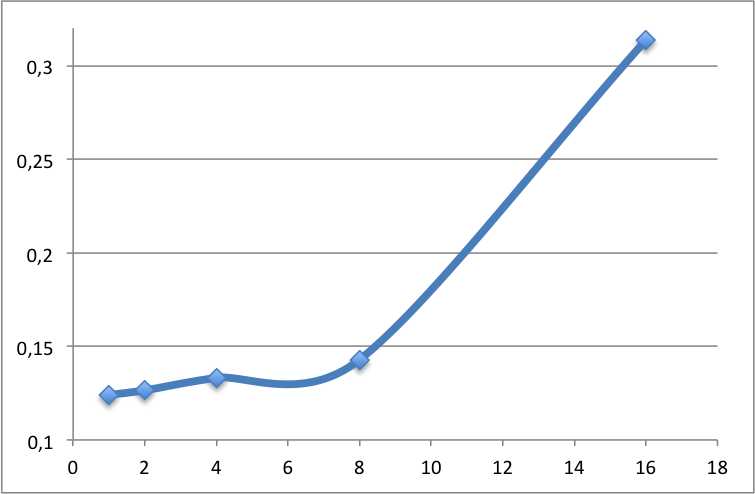
\includegraphics{processor_scale.png}
  \caption{Increasing the number of nodes, same size and initial number of particles}
  \label{fig1}
\end{figure}

The increase of number of particles gives an exponential growth of the
execution time. This is because of the need for neighbor-checking,
which means that a double amount of particles also means a double amount
of neighbors to check for each particle, on average. We can see this in
Figure \ref{fig2}.\\

\begin{figure}
  \centering
  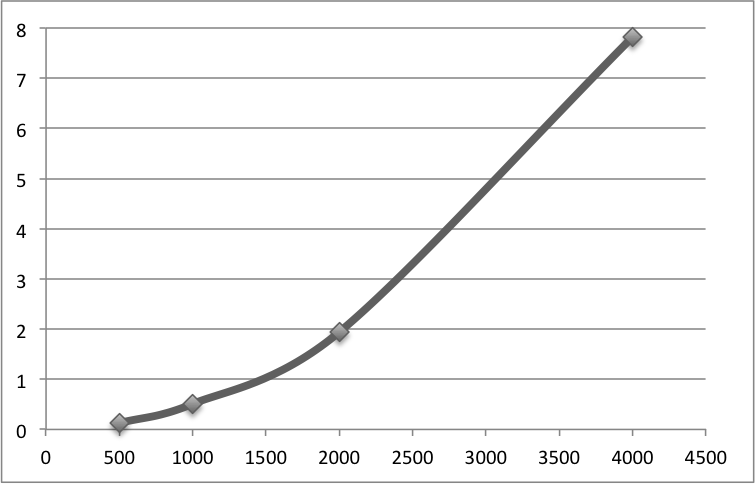
\includegraphics{particles_scale.png}
  \caption{Increasing the number of initial particles, same size and number of nodes}
  \label{fig2}
\end{figure}

\subsection{Changing area size}

Changing the size of the area does not affect the runtime very much. We
have noticed that a smaller area takes slightly longer time than a
larger box, which is natural since particles will collide with walls and
to travel between nodes more often than in large boxes.\\


\end{document}
